\problemname{Buying a Rug}
\begin{center}
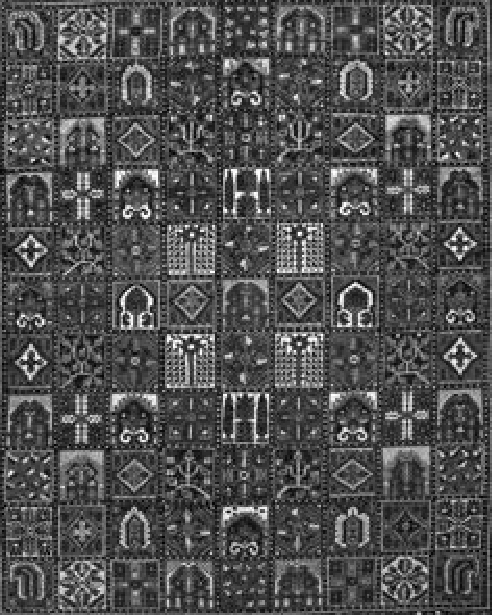
\includegraphics[width=4cm]{matta.pdf}
\end{center}

During IOI in Tehran this summer, there was an increased demand for Persian
rugs, particularly those with a pattern consisting of a grid of $L
\times B$ squares (see image above), since these are very suitable for
secretly trying out algorithms on.

A rug's price is usually determined by the number of squares, so a typical customer wants
a rug with at least $M$ squares and at most $N$ squares. If there are several
possible rugs, the customer wants one as square as possible,
i.e.\ they want $|L - B|$ to be as small as possible.

Write a program that reads the numbers $M$ and $N$ and outputs the
best choice of $B$ and $L$.

\section*{Input}

One line with two integers $M$ and $N$.

\section*{Output}

Output the numbers $B$ and $L$ (the smallest side length first). For the given input, the answer is uniquely determined.

\section*{Scoring}
For test cases worth $40$ points, $1 \le M \le N \le 1\,000$. \\
For test cases worth $20$ points, $M = N$ and $10^{11} \le M \le 10^{12}$. \\
For test cases worth $40$ points, $10^8 \le M \le N \le 10^{12}$.
